
\section{Campo de batalla}
En esta sección veremos los tipos de terrenos que se han utilizado, cómo se han usado y cual será su forma de afectar al movimiento de los personajes. El mapa de juego se ha creado en forma de \textit{grid} donde cada celda del \textit{grid} tendrá una etiqueta de tipo \textit{Floor} y una textura que permita distinguir el tipo de terreno. En total se han utilizado 10 tipos distintos de terrenos:
\begin{enumerate}
    \item Piedra gris: La piedra gris permite tanto delimitar los bordes de las bases como los pasos entre zonas. Es un material por el que a priori los personajes no tienen mayor dificultad para andar, exceptuando las unidades con montura que pueden resbalar en el por lo que deberían reducir su velocidad.  
    \item Camino marrón claro y marrón oscuro: Estos dos materiales son usados para crear calzadas por las que las unidades terrestres gustan andar y a priori todas podrán andar por estos caminos teniendo en cuenta que unas tendrán preferencia por el marrón y otras por el marrón claro. Las preferencias de movimiento se verán más adelante.
    \item Pradera: Es una zona en donde las unidades pesadas encontrarán dificultad para moverse, pero otro tipo de unidades más ligeras, en especial las unidades a distancia encontrarán facilidad de movimiento y sitio para atacar a unidades que puedan encontrarse en los caminos.
    \item Arena clara y oscura: Estas texturas formarán zonas de dunas de arena en donde la mayoría de unidades verán reducido su movimiento pero tendrán que atravesar si quieren conseguir algún sub-objetivo o zona de curación. 
    \item Agua: Las zonas de agua oscura serán las más profundas y que ninguna unidad será capaz de atravesar. Sin embargo, el agua más clara y menos profunda puede ser atravesada por unidades montadas o unidades ligeras, ya que las más pesadas pueden ser susceptibles de hundirse aquí.
    \item Suelo: Las zonas de suelo ajedrezadas indicarán dónde se sitúan las bases  
    \item Lava: Terreno al que las unidades suelen dar muy poca preferencia ya que reduce considerablemente la velocidad de movimiento.
\end{enumerate}
El terreno de juego como podemos ver en \ref{fig:mapa} está formado por un grid de 52x52 donde se han representado 2 bases, la del equipo A en la zona inferior y el equipo B en la zona superior. Estas bases están separadas por un río que no se puede cruzar y conectadas por 3 puentes. Cada base está conectada por una serie de caminos hacia la base enemiga, encontrándose zonas de interés como zonas de curación.
 \begin{figure}[H]
    \centering
    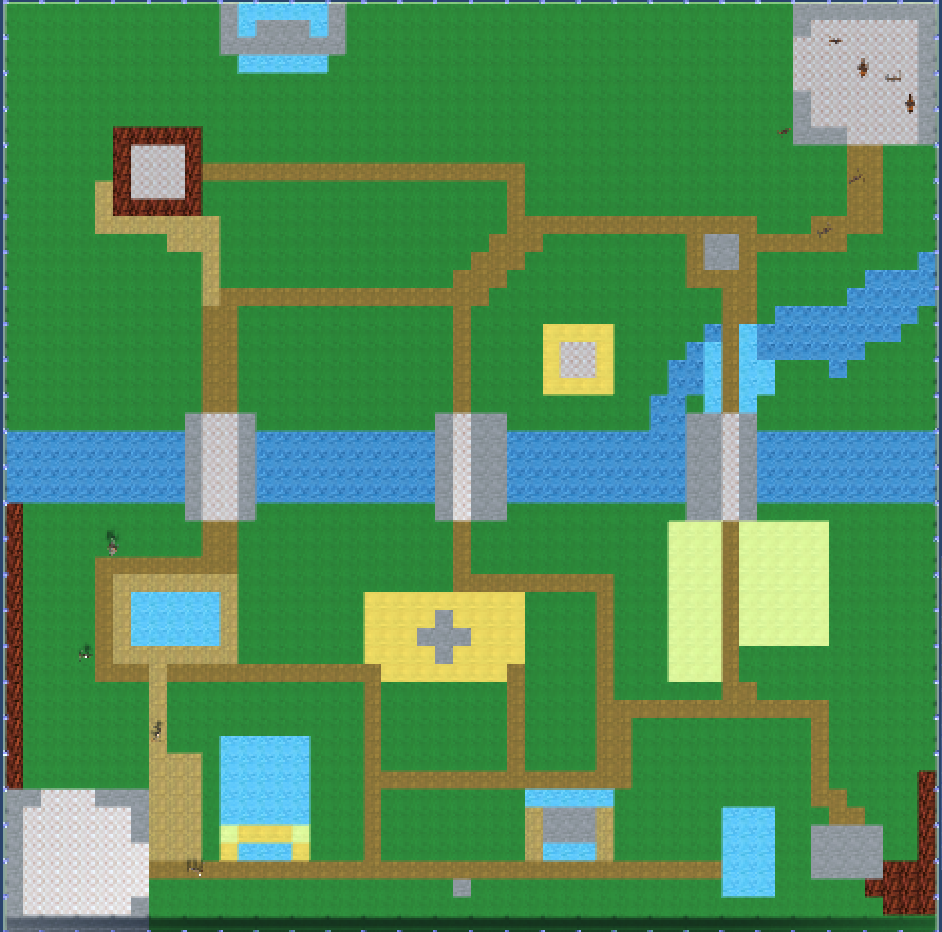
\includegraphics[scale=0.7]{doc/images/Mapa.png}
    \caption{Terreno de juego}
    \label{fig:mapa}
\end{figure}
\section{Tipos de Unidades}
Al habernos basado en un juego de captura de bases tipo RTS lo suyo era tener varias unidades que tengan movimientos variados dependiendo del terreno y de los personajes que se encuentren para pelear. Es por esto que se han implementando 4 tipos de unidades:
Unidades de infantería, unidad a caballo, Unidad Arquera y Unidad Lancera. Para distinguir las unidades se han usado unos assets de la store de unity .
\footnote{Toon RTS Units 3D \url{https://assetstore.unity.com/packages/3d/characters/toon-rts-units-67948}.}

Por cada unidad tendremos una clase distinta que hereda de la clase AgentNPC. En cada una de estas clases hija tendremos una estructura de tipo diccionario $<$Terreno, Float$>$ donde a cada tipo de terreno se le asignará un multiplicador de influencia para cada personaje, los cuales se utilizarán en el comportamiento táctico de las unidades que veremos más adelante.\\

La clase AgentNPC definirá todos los atributos de un personaje como pueden ser la vida, velocidad de movimiento, ataque, etc y serán las clases hijas las encargadas de asignar valores a estos atributos en función de las características que se les quieran asignar. Además tenemos el método \textit{GenerateCostsDict} en cada clase de unidad, que será llamado en el método \textit{Start}, donde se asigna a cada tipo de terreno un multiplicador de coste de movimiento para ese personaje, veamos como quedaría en el caso de la Unidad Lancero la asignación de influencia e inicialización de atributos:
\begin{lstlisting}
    private new void Start()
    {
        base.Start();
        _mass = 4f;
        _maxSpeed = 7f;
        _maxRotation = 5f;
        _maxAcceleration = 4f;
        _maxAngularAcc = 10f;
        _maxForce = 3f;
        _baseDamage = 30f;
        _attackRange = 2f;
        _attackSpeed = 2f;
        _hpMax = 130;
        _hpCurrent = 130;
        
        GenerateCostsDict();
    }
    } \end{lstlisting}
\begin{lstlisting}

    private void GenerateCostsDict()
    {
        terrainCosts.Add(TerrainType.Grass, 1f);
        terrainCosts.Add(TerrainType.Stones, 1.5f);
        terrainCosts.Add(TerrainType.Floor, 5f);
        terrainCosts.Add(TerrainType.Sand, 10f);
        terrainCosts.Add(TerrainType.Lava, 15f);
        terrainCosts.Add(TerrainType.Water, Mathf.Infinity);
    } \end{lstlisting}

%TBD EDITAR
En el método update de la clase AgentNpc antes de aplicar los steerings se recalculará la velocidad de movimiento en función del terreno   sobre el que esté el personaje:
\begin{lstlisting}
 public new void Update()
    {
        String textureName;
        base.Update();
        Ray NpcPos = Camera.main.ScreenPointToRay(Position);
        RaycastHit hitInfo;
        if (Physics.Raycast(NpcPos, out hitInfo) && hitInfo.collider != null)
        {

            if (hitInfo.collider.CompareTag("Floor"))
            {
             textureName = hitInfo.collider.gameObject.GetComponent<MeshRenderer>().material.mainTexture.name;
            _maxSpeed = _maxSpeed / _costes[getTerreno(textureName)];

            }
        }
        ApplySteering();
    }
\end{lstlisting}

El método \textit{getTerreno} simplemente devolverá el tipo de terreno en función del nombre de la textura detectada.\\

En la siguiente tabla podemos ver una relación de los tipos de unidades y su multiplicador de velocidad según el terreno. También veremos otra tabla con los distintos valores de influencia dependiendo del terreno y la unidad.

\begin{table}[H]
    \centering
    \begin{tabular}{|c|c|c|c|c|}
        \cline{2-5}        
        \multicolumn{1}{c|}{} & 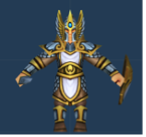
\includegraphics{imagesTable/infanteria} & 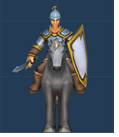
\includegraphics{imagesTable/caballo} & 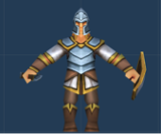
\includegraphics{imagesTable/lancero} & 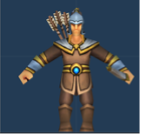
\includegraphics{imagesTable/arquero} \\
        \hline
        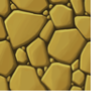
\includegraphics{imagesTable/claroPiedra} 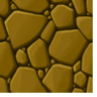
\includegraphics{imagesTable/piedra} 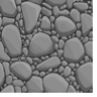
\includegraphics{imagesTable/grisPiedra} & 1.5 & 1.5 & 1.5 & 1.5 \\
        \hline
        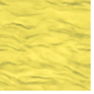
\includegraphics{imagesTable/arena} 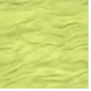
\includegraphics{imagesTable/claroArena} & 10 & 10 & 3 & 3 \\
        \hline
        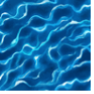
\includegraphics{imagesTable/agua} 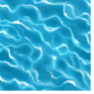
\includegraphics{imagesTable/claroAgua} & $\infty$ & $\infty$  & $\infty$ & $\infty$ \\
        \hline
        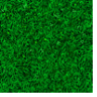
\includegraphics{imagesTable/hierba} & 5 & 1 & 5 & 1 \\
        \hline
        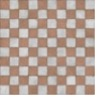
\includegraphics[scale=0.5]{imagesTable/suelo} & 1 & 5 & 1 & 1 \\
        \hline
        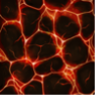
\includegraphics{imagesTable/lava} & 15 & 15 & 15 & 15 \\
        \hline
    \end{tabular}
    \caption{Tabla de Influencias}
\end{table}
%TBD RELLENAR VALORES VELOCIDADES
\begin{table}[H]
    \centering
    \begin{tabular}{|c|c|c|c|c|}
        \cline{2-5}        
        \multicolumn{1}{c|}{} & 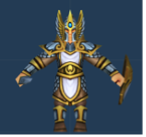
\includegraphics{imagesTable/infanteria} & 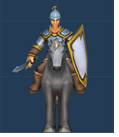
\includegraphics{imagesTable/caballo} & 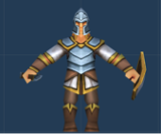
\includegraphics{imagesTable/lancero} & 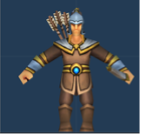
\includegraphics{imagesTable/arquero} \\
        \hline
        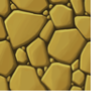
\includegraphics{imagesTable/claroPiedra} 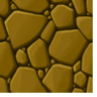
\includegraphics{imagesTable/piedra} 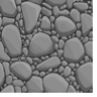
\includegraphics{imagesTable/grisPiedra} & 75\% & 75\% & 90\% & 90\% \\
        \hline
        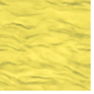
\includegraphics{imagesTable/arena} 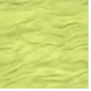
\includegraphics{imagesTable/claroArena} & 25\% & 25\% & 60\% & 60\% \\
        \hline
        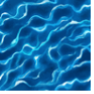
\includegraphics{imagesTable/agua} 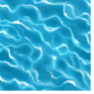
\includegraphics{imagesTable/claroAgua} & 0\% & 0\% & 0\% & 0\% \\
        \hline
        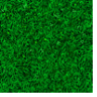
\includegraphics{imagesTable/hierba} & 50\% & 100\% & 45\% & 100\% \\
        \hline
        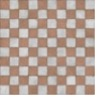
\includegraphics[scale=0.5]{imagesTable/suelo} & 100\% & 50\% & 100\% & 100\% \\
        \hline
        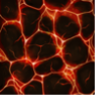
\includegraphics{imagesTable/lava} & 5\% & 5\% & 10\% & 2\% \\
        \hline
    \end{tabular}
    \caption{Tabla de velocidades}
\end{table}


